\documentclass[twoside]{book}

% Packages required by doxygen
\usepackage{fixltx2e}
\usepackage{calc}
\usepackage{doxygen}
\usepackage[export]{adjustbox} % also loads graphicx
\usepackage{graphicx}
\usepackage[utf8]{inputenc}
\usepackage{makeidx}
\usepackage{multicol}
\usepackage{multirow}
\PassOptionsToPackage{warn}{textcomp}
\usepackage{textcomp}
\usepackage[nointegrals]{wasysym}
\usepackage[table]{xcolor}

% Font selection
\usepackage[T1]{fontenc}
\usepackage[scaled=.90]{helvet}
\usepackage{courier}
\usepackage{amssymb}
\usepackage{sectsty}
\renewcommand{\familydefault}{\sfdefault}
\allsectionsfont{%
  \fontseries{bc}\selectfont%
  \color{darkgray}%
}
\renewcommand{\DoxyLabelFont}{%
  \fontseries{bc}\selectfont%
  \color{darkgray}%
}
\newcommand{\+}{\discretionary{\mbox{\scriptsize$\hookleftarrow$}}{}{}}

% Page & text layout
\usepackage{geometry}
\geometry{%
  a4paper,%
  top=2.5cm,%
  bottom=2.5cm,%
  left=2.5cm,%
  right=2.5cm%
}
\tolerance=750
\hfuzz=15pt
\hbadness=750
\setlength{\emergencystretch}{15pt}
\setlength{\parindent}{0cm}
\setlength{\parskip}{3ex plus 2ex minus 2ex}
\makeatletter
\renewcommand{\paragraph}{%
  \@startsection{paragraph}{4}{0ex}{-1.0ex}{1.0ex}{%
    \normalfont\normalsize\bfseries\SS@parafont%
  }%
}
\renewcommand{\subparagraph}{%
  \@startsection{subparagraph}{5}{0ex}{-1.0ex}{1.0ex}{%
    \normalfont\normalsize\bfseries\SS@subparafont%
  }%
}
\makeatother

% Headers & footers
\usepackage{fancyhdr}
\pagestyle{fancyplain}
\fancyhead[LE]{\fancyplain{}{\bfseries\thepage}}
\fancyhead[CE]{\fancyplain{}{}}
\fancyhead[RE]{\fancyplain{}{\bfseries\leftmark}}
\fancyhead[LO]{\fancyplain{}{\bfseries\rightmark}}
\fancyhead[CO]{\fancyplain{}{}}
\fancyhead[RO]{\fancyplain{}{\bfseries\thepage}}
\fancyfoot[LE]{\fancyplain{}{}}
\fancyfoot[CE]{\fancyplain{}{}}
\fancyfoot[RE]{\fancyplain{}{\bfseries\scriptsize Generated by Doxygen }}
\fancyfoot[LO]{\fancyplain{}{\bfseries\scriptsize Generated by Doxygen }}
\fancyfoot[CO]{\fancyplain{}{}}
\fancyfoot[RO]{\fancyplain{}{}}
\renewcommand{\footrulewidth}{0.4pt}
\renewcommand{\chaptermark}[1]{%
  \markboth{#1}{}%
}
\renewcommand{\sectionmark}[1]{%
  \markright{\thesection\ #1}%
}

% Indices & bibliography
\usepackage{natbib}
\usepackage[titles]{tocloft}
\setcounter{tocdepth}{3}
\setcounter{secnumdepth}{5}
\makeindex

% Hyperlinks (required, but should be loaded last)
\usepackage{ifpdf}
\ifpdf
  \usepackage[pdftex,pagebackref=true]{hyperref}
\else
  \usepackage[ps2pdf,pagebackref=true]{hyperref}
\fi
\hypersetup{%
  colorlinks=true,%
  linkcolor=blue,%
  citecolor=blue,%
  unicode%
}

% Custom commands
\newcommand{\clearemptydoublepage}{%
  \newpage{\pagestyle{empty}\cleardoublepage}%
}

\usepackage{caption}
\captionsetup{labelsep=space,justification=centering,font={bf},singlelinecheck=off,skip=4pt,position=top}

%===== C O N T E N T S =====

\begin{document}

% Titlepage & ToC
\hypersetup{pageanchor=false,
             bookmarksnumbered=true,
             pdfencoding=unicode
            }
\pagenumbering{roman}
\begin{titlepage}
\vspace*{7cm}
\begin{center}%
{\Large Tomato }\\
\vspace*{1cm}
{\large Generated by Doxygen 1.8.11}\\
\end{center}
\end{titlepage}
\clearemptydoublepage
\tableofcontents
\clearemptydoublepage
\pagenumbering{arabic}
\hypersetup{pageanchor=true}

%--- Begin generated contents ---
\chapter{Code of Conduct}
\label{md_codeofconduct}
\hypertarget{md_codeofconduct}{}
\input{md_codeofconduct}
\chapter{Contributing to T\+O\+M\+A\+TO}
\label{md_contributing}
\hypertarget{md_contributing}{}
\input{md_contributing}
\chapter{T\+O\+M\+A\+TO}
\label{md_README}
\hypertarget{md_README}{}
T\+O\+M\+A\+TO (Total Mapping Toolbox) is a C++ library for the calculation of parametric maps in cardiac magnetic resonance imaging (M\+RI). As an open source project, T\+O\+M\+A\+TO allows transparent and standardized cardiac longitudinal relaxation time (T1) mapping in clinical applications. With C++ implementation, T\+O\+M\+A\+TO can easily interface and translate between research software environments, and commercial vendors’ closed-\/source C++ environments on scanners as well as post-\/processing software. To complement the core library implementation, a ready-\/to-\/use command line tool has been provided.

It contains Sh\+M\+O\+L\+LI implementation as in \href{https://jcmr-online.biomedcentral.com/articles/10.1186/1532-429X-12-69}{\tt this article}.

\tabulinesep=1mm
\begin{longtabu} spread 0pt [c]{*2{|X[-1]}|}
\hline
\rowcolor{\tableheadbgcolor}{\bf System }&\PBS\centering {\bf Status  }\\\cline{1-2}
\endfirsthead
\hline
\endfoot
\hline
\rowcolor{\tableheadbgcolor}{\bf System }&\PBS\centering {\bf Status  }\\\cline{1-2}
\endhead
\+:tomato\+: \href{https://mrkonrad.github.io/tomato_docs/}{\tt Tutorial} \+:tomato\+: &\PBS\centering \+:tomato\+: \href{https://mrkonrad.github.io/tomato_docs/}{\tt Tomato Docs} \+:tomato\+: \\\cline{1-2}
\href{https://mrkonrad.github.io/tomato/html/md__r_e_a_d_m_e.html}{\tt Code documentation} &\PBS\centering \href{https://mrkonrad.github.io/tomato/html/md__r_e_a_d_m_e.html}{\tt Doxygen} \\\cline{1-2}
\href{https://doi.org/10.1016/j.softx.2019.100369}{\tt D\+OI} &\PBS\centering \href{https://doi.org/10.1016/j.softx.2019.100369}{\tt } \\\cline{1-2}
\href{https://travis-ci.org/MRKonrad/tomato}{\tt O\+S\+X/\+Linux build -\/ Travis} &\PBS\centering \href{https://travis-ci.org/MRKonrad/tomato}{\tt } \\\cline{1-2}
\href{https://ci.appveyor.com/project/MRKonrad/tomato}{\tt Windows build -\/ App\+Veyor} &\PBS\centering \href{https://ci.appveyor.com/project/MRKonrad/tomato}{\tt } \\\cline{1-2}
\href{https://codecov.io/gh/MRKonrad/tomato}{\tt Test coverage -\/ Codecov} &\PBS\centering \href{https://codecov.io/gh/MRKonrad/tomato}{\tt } \\\cline{1-2}
\href{https://github.com/MRKonrad/tomato/releases}{\tt Downloads} &\PBS\centering \href{https://github.com/MRKonrad/tomato/releases}{\tt } \\\cline{1-2}
\end{longtabu}
\subsection*{How to compile}

\href{cmake.org}{\tt C\+Make} build system and \href{conan.io}{\tt Conan} cpp package manager are recommended.


\begin{DoxyEnumerate}
\item Get dependencies In the conan-\/recipes folder\+: ```bash conan create conan-\/gtest-\/1.\+8.\+1 user/testing conan create conan-\/vxl-\/2.\+0.\+2 user/testing conan create libyaml user/testing conan create lmfit user/testing ```
\item Build In the source folder\+: ```bash mkdir build cd build conan install .. cmake .. cmake --build . cmake --build --target I\+N\+S\+T\+A\+LL ```
\end{DoxyEnumerate}

\subsection*{Tomato\+Open\+Source and Tomato\+Full}

{\bfseries Important}

There are two {\ttfamily Tomato} version available\+: {\ttfamily Tomato\+Open\+Source} compiled with publicly available code and {\ttfamily Tomato\+Full} containing additionally private code used for {\ttfamily Amoeba\+Private\+Nr2} fitting algorithm using Nelder–\+Mead algorithm based on Numerical Recipes. Original Sh\+M\+O\+L\+LI (and based on it Tomato) uses code based on Numerical Recipes book. Due to Numerical Recipes licence I cannot share this part of the code online. Please contact me if you would like to use this part of the code. To make up for this limitation we provide a number of alternative fitting procedures.

\subsection*{Contributing and code of conduct}

Please see \hyperlink{md_contributing}{contributing.md} and \hyperlink{md_codeofconduct}{codeofconduct.md}.

\subsection*{Troubleshooting}


\begin{DoxyItemize}
\item Problem\+: missing msvcp140.\+dll
\item Solution\+: Download \href{https://www.microsoft.com/en-us/download/details.aspx?id=48145}{\tt https\+://www.\+microsoft.\+com/en-\/us/download/details.\+aspx?id=48145} as suggested in \href{https://stackoverflow.com/questions/32998902/msvcp140-dll-missing}{\tt https\+://stackoverflow.\+com/questions/32998902/msvcp140-\/dll-\/missing} 
\end{DoxyItemize}
\chapter{Hierarchical Index}
\input{hierarchy}
\chapter{Class Index}
\input{annotated}
\chapter{File Index}
\section{File List}
Here is a list of all documented files with brief descriptions\+:\begin{DoxyCompactList}
\item\contentsline{section}{lib/{\bfseries gdcm\+Tomato\+Read\+Tags.\+h} }{\pageref{gdcm_tomato_read_tags_8h}}{}
\item\contentsline{section}{lib/\hyperlink{itk_calculator_t1_image_filter_8h}{itk\+Calculator\+T1\+Image\+Filter.\+h} }{\pageref{itk_calculator_t1_image_filter_8h}}{}
\item\contentsline{section}{lib/\hyperlink{itk_calculator_t1_image_filter_8hxx}{itk\+Calculator\+T1\+Image\+Filter.\+hxx} }{\pageref{itk_calculator_t1_image_filter_8hxx}}{}
\item\contentsline{section}{lib/{\bfseries itk\+Colorbar2\+D\+Image\+Filter.\+h} }{\pageref{itk_colorbar2_d_image_filter_8h}}{}
\item\contentsline{section}{lib/{\bfseries itk\+Image\+File\+Reader\+K\+W.\+h} }{\pageref{itk_image_file_reader_k_w_8h}}{}
\item\contentsline{section}{lib/{\bfseries itk\+Image\+File\+Reader\+K\+W.\+hxx} }{\pageref{itk_image_file_reader_k_w_8hxx}}{}
\item\contentsline{section}{lib/{\bfseries itk\+N\+Shmolli\+Samples\+Used\+To123\+Image\+Filter.\+h} }{\pageref{itk_n_shmolli_samples_used_to123_image_filter_8h}}{}
\item\contentsline{section}{lib/{\bfseries itk\+Read\+File\+List\+Filter.\+h} }{\pageref{itk_read_file_list_filter_8h}}{}
\item\contentsline{section}{lib/{\bfseries itk\+Read\+File\+List\+Filter.\+hxx} }{\pageref{itk_read_file_list_filter_8hxx}}{}
\item\contentsline{section}{lib/{\bfseries itk\+Sort\+Inv\+Times\+Image\+Filter.\+h} }{\pageref{itk_sort_inv_times_image_filter_8h}}{}
\item\contentsline{section}{lib/{\bfseries K\+W\+Util.\+h} }{\pageref{_k_w_util_8h}}{}
\item\contentsline{section}{lib/{\bfseries K\+W\+Util.\+hxx} }{\pageref{_k_w_util_8hxx}}{}
\item\contentsline{section}{lib/\hyperlink{_k_w_util_yaml_8h}{K\+W\+Util\+Yaml.\+h} }{\pageref{_k_w_util_yaml_8h}}{}
\item\contentsline{section}{lib/\hyperlink{_ox_calculator_8h}{Ox\+Calculator.\+h} }{\pageref{_ox_calculator_8h}}{}
\item\contentsline{section}{lib/\hyperlink{_ox_calculator_8hxx}{Ox\+Calculator.\+hxx} }{\pageref{_ox_calculator_8hxx}}{}
\item\contentsline{section}{lib/\hyperlink{_ox_calculator_t1_shmolli_8h}{Ox\+Calculator\+T1\+Shmolli.\+h} }{\pageref{_ox_calculator_t1_shmolli_8h}}{}
\item\contentsline{section}{lib/\hyperlink{_ox_calculator_t1_shmolli_8hxx}{Ox\+Calculator\+T1\+Shmolli.\+hxx} }{\pageref{_ox_calculator_t1_shmolli_8hxx}}{}
\item\contentsline{section}{lib/\hyperlink{_ox_calculator_t1_with_sign_check_8h}{Ox\+Calculator\+T1\+With\+Sign\+Check.\+h} }{\pageref{_ox_calculator_t1_with_sign_check_8h}}{}
\item\contentsline{section}{lib/\hyperlink{_ox_calculator_t1_with_sign_check_8hxx}{Ox\+Calculator\+T1\+With\+Sign\+Check.\+hxx} }{\pageref{_ox_calculator_t1_with_sign_check_8hxx}}{}
\item\contentsline{section}{lib/\hyperlink{_ox_factory_of_calculators_8h}{Ox\+Factory\+Of\+Calculators.\+h} }{\pageref{_ox_factory_of_calculators_8h}}{}
\item\contentsline{section}{lib/\hyperlink{_ox_factory_of_calculators_8hxx}{Ox\+Factory\+Of\+Calculators.\+hxx} }{\pageref{_ox_factory_of_calculators_8hxx}}{}
\item\contentsline{section}{lib/\hyperlink{_ox_factory_of_fitters_8h}{Ox\+Factory\+Of\+Fitters.\+h} }{\pageref{_ox_factory_of_fitters_8h}}{}
\item\contentsline{section}{lib/\hyperlink{_ox_factory_of_fitters_8hxx}{Ox\+Factory\+Of\+Fitters.\+hxx} }{\pageref{_ox_factory_of_fitters_8hxx}}{}
\item\contentsline{section}{lib/{\bfseries Ox\+Factory\+Of\+Models.\+h} }{\pageref{_ox_factory_of_models_8h}}{}
\item\contentsline{section}{lib/{\bfseries Ox\+Factory\+Of\+Models.\+hxx} }{\pageref{_ox_factory_of_models_8hxx}}{}
\item\contentsline{section}{lib/\hyperlink{_ox_factory_of_sign_calculators_8h}{Ox\+Factory\+Of\+Sign\+Calculators.\+h} }{\pageref{_ox_factory_of_sign_calculators_8h}}{}
\item\contentsline{section}{lib/\hyperlink{_ox_factory_of_sign_calculators_8hxx}{Ox\+Factory\+Of\+Sign\+Calculators.\+hxx} }{\pageref{_ox_factory_of_sign_calculators_8hxx}}{}
\item\contentsline{section}{lib/\hyperlink{_ox_factory_of_start_point_calculators_8h}{Ox\+Factory\+Of\+Start\+Point\+Calculators.\+h} }{\pageref{_ox_factory_of_start_point_calculators_8h}}{}
\item\contentsline{section}{lib/\hyperlink{_ox_factory_of_start_point_calculators_8hxx}{Ox\+Factory\+Of\+Start\+Point\+Calculators.\+hxx} }{\pageref{_ox_factory_of_start_point_calculators_8hxx}}{}
\item\contentsline{section}{lib/\hyperlink{_ox_fitter_8h}{Ox\+Fitter.\+h} }{\pageref{_ox_fitter_8h}}{}
\item\contentsline{section}{lib/\hyperlink{_ox_fitter_amoeba_nr2_8h}{Ox\+Fitter\+Amoeba\+Nr2.\+h} }{\pageref{_ox_fitter_amoeba_nr2_8h}}{}
\item\contentsline{section}{lib/\hyperlink{_ox_fitter_amoeba_vnl_8h}{Ox\+Fitter\+Amoeba\+Vnl.\+h} }{\pageref{_ox_fitter_amoeba_vnl_8h}}{}
\item\contentsline{section}{lib/{\bfseries Ox\+Fitter\+Amoeba\+Vnl.\+hxx} }{\pageref{_ox_fitter_amoeba_vnl_8hxx}}{}
\item\contentsline{section}{lib/\hyperlink{_ox_fitter_levenberg_marquardt_lmfit_8h}{Ox\+Fitter\+Levenberg\+Marquardt\+Lmfit.\+h} }{\pageref{_ox_fitter_levenberg_marquardt_lmfit_8h}}{}
\item\contentsline{section}{lib/{\bfseries Ox\+Fitter\+Levenberg\+Marquardt\+Lmfit.\+hxx} }{\pageref{_ox_fitter_levenberg_marquardt_lmfit_8hxx}}{}
\item\contentsline{section}{lib/\hyperlink{_ox_fitter_levenberg_marquardt_vnl_8h}{Ox\+Fitter\+Levenberg\+Marquardt\+Vnl.\+h} }{\pageref{_ox_fitter_levenberg_marquardt_vnl_8h}}{}
\item\contentsline{section}{lib/{\bfseries Ox\+Fitter\+Levenberg\+Marquardt\+Vnl.\+hxx} }{\pageref{_ox_fitter_levenberg_marquardt_vnl_8hxx}}{}
\item\contentsline{section}{lib/\hyperlink{_ox_image_calculator_8h}{Ox\+Image\+Calculator.\+h} }{\pageref{_ox_image_calculator_8h}}{}
\item\contentsline{section}{lib/\hyperlink{_ox_image_calculator_8hxx}{Ox\+Image\+Calculator.\+hxx} }{\pageref{_ox_image_calculator_8hxx}}{}
\item\contentsline{section}{lib/\hyperlink{_ox_model_8h}{Ox\+Model.\+h} }{\pageref{_ox_model_8h}}{}
\item\contentsline{section}{lib/{\bfseries Ox\+Model.\+hxx} }{\pageref{_ox_model_8hxx}}{}
\item\contentsline{section}{lib/\hyperlink{_ox_model_t1_adapter_lmfit_least_squares_8h}{Ox\+Model\+T1\+Adapter\+Lmfit\+Least\+Squares.\+h} }{\pageref{_ox_model_t1_adapter_lmfit_least_squares_8h}}{}
\item\contentsline{section}{lib/\hyperlink{_ox_model_t1_adapter_tomato_fit_least_squares_8h}{Ox\+Model\+T1\+Adapter\+Tomato\+Fit\+Least\+Squares.\+h} }{\pageref{_ox_model_t1_adapter_tomato_fit_least_squares_8h}}{}
\item\contentsline{section}{lib/\hyperlink{_ox_model_t1_adapter_vnl_cost_8h}{Ox\+Model\+T1\+Adapter\+Vnl\+Cost.\+h} }{\pageref{_ox_model_t1_adapter_vnl_cost_8h}}{}
\item\contentsline{section}{lib/\hyperlink{_ox_model_t1_adapter_vnl_least_squares_8h}{Ox\+Model\+T1\+Adapter\+Vnl\+Least\+Squares.\+h} }{\pageref{_ox_model_t1_adapter_vnl_least_squares_8h}}{}
\item\contentsline{section}{lib/\hyperlink{_ox_model_t1_shmolli_8h}{Ox\+Model\+T1\+Shmolli.\+h} }{\pageref{_ox_model_t1_shmolli_8h}}{}
\item\contentsline{section}{lib/\hyperlink{_ox_model_t1_shmolli_8hxx}{Ox\+Model\+T1\+Shmolli.\+hxx} }{\pageref{_ox_model_t1_shmolli_8hxx}}{}
\item\contentsline{section}{lib/\hyperlink{_ox_model_t1_three_param_8h}{Ox\+Model\+T1\+Three\+Param.\+h} }{\pageref{_ox_model_t1_three_param_8h}}{}
\item\contentsline{section}{lib/\hyperlink{_ox_model_t1_three_param_8hxx}{Ox\+Model\+T1\+Three\+Param.\+hxx} }{\pageref{_ox_model_t1_three_param_8hxx}}{}
\item\contentsline{section}{lib/\hyperlink{_ox_model_t1_two_param_8h}{Ox\+Model\+T1\+Two\+Param.\+h} }{\pageref{_ox_model_t1_two_param_8h}}{}
\item\contentsline{section}{lib/\hyperlink{_ox_model_t1_two_param_8hxx}{Ox\+Model\+T1\+Two\+Param.\+hxx} }{\pageref{_ox_model_t1_two_param_8hxx}}{}
\item\contentsline{section}{lib/\hyperlink{_ox_original_shmolli_dicom_reader_8h}{Ox\+Original\+Shmolli\+Dicom\+Reader.\+h} }{\pageref{_ox_original_shmolli_dicom_reader_8h}}{}
\item\contentsline{section}{lib/\hyperlink{_ox_original_shmolli_dicom_reader_8hxx}{Ox\+Original\+Shmolli\+Dicom\+Reader.\+hxx} }{\pageref{_ox_original_shmolli_dicom_reader_8hxx}}{}
\item\contentsline{section}{lib/\hyperlink{_ox_sign_calculator_8h}{Ox\+Sign\+Calculator.\+h} }{\pageref{_ox_sign_calculator_8h}}{}
\item\contentsline{section}{lib/\hyperlink{_ox_sign_calculator_no_sign_8h}{Ox\+Sign\+Calculator\+No\+Sign.\+h} }{\pageref{_ox_sign_calculator_no_sign_8h}}{}
\item\contentsline{section}{lib/\hyperlink{_ox_sign_calculator_real_imag_8h}{Ox\+Sign\+Calculator\+Real\+Imag.\+h} }{\pageref{_ox_sign_calculator_real_imag_8h}}{}
\item\contentsline{section}{lib/\hyperlink{_ox_sign_calculator_shmolli_8h}{Ox\+Sign\+Calculator\+Shmolli.\+h} }{\pageref{_ox_sign_calculator_shmolli_8h}}{}
\item\contentsline{section}{lib/\hyperlink{_ox_start_point_calculator_8h}{Ox\+Start\+Point\+Calculator.\+h} }{\pageref{_ox_start_point_calculator_8h}}{}
\item\contentsline{section}{lib/\hyperlink{_ox_start_point_calculator_basic_8h}{Ox\+Start\+Point\+Calculator\+Basic.\+h} }{\pageref{_ox_start_point_calculator_basic_8h}}{}
\item\contentsline{section}{lib/\hyperlink{_ox_start_point_calculator_shmolli_8h}{Ox\+Start\+Point\+Calculator\+Shmolli.\+h} }{\pageref{_ox_start_point_calculator_shmolli_8h}}{}
\item\contentsline{section}{lib/\hyperlink{_tomato_8h}{Tomato.\+h} }{\pageref{_tomato_8h}}{}
\item\contentsline{section}{lib/{\bfseries Tomato.\+hxx} }{\pageref{_tomato_8hxx}}{}
\item\contentsline{section}{lib/\hyperlink{_tomato__export_t1_8hxx}{Tomato\+\_\+export\+T1.\+hxx} }{\pageref{_tomato__export_t1_8hxx}}{}
\item\contentsline{section}{lib/{\bfseries Tomato\+\_\+export\+T1\+\_\+mag\+Sign\+Recov.\+hxx} }{\pageref{_tomato__export_t1__mag_sign_recov_8hxx}}{}
\item\contentsline{section}{lib/\hyperlink{_tomato__export_t2_8hxx}{Tomato\+\_\+export\+T2.\+hxx} }{\pageref{_tomato__export_t2_8hxx}}{}
\item\contentsline{section}{lib/\hyperlink{_tomato_api_8cpp}{Tomato\+Api.\+cpp} }{\pageref{_tomato_api_8cpp}}{}
\item\contentsline{section}{lib/\hyperlink{_tomato_api_8h}{Tomato\+Api.\+h} }{\pageref{_tomato_api_8h}}{}
\item\contentsline{section}{lib/\hyperlink{_tomato_colormap_8cpp}{Tomato\+Colormap.\+cpp} }{\pageref{_tomato_colormap_8cpp}}{}
\item\contentsline{section}{lib/\hyperlink{_tomato_colormap_8h}{Tomato\+Colormap.\+h} }{\pageref{_tomato_colormap_8h}}{}
\item\contentsline{section}{lib/\hyperlink{_tomato_one_pixel_8h}{Tomato\+One\+Pixel.\+h} }{\pageref{_tomato_one_pixel_8h}}{}
\item\contentsline{section}{lib/\hyperlink{_tomato_options_8h}{Tomato\+Options.\+h} }{\pageref{_tomato_options_8h}}{}
\item\contentsline{section}{lib/\hyperlink{_tomato_options_8hxx}{Tomato\+Options.\+hxx} }{\pageref{_tomato_options_8hxx}}{}
\item\contentsline{section}{lib/\hyperlink{_tomato_parser_8h}{Tomato\+Parser.\+h} }{\pageref{_tomato_parser_8h}}{}
\item\contentsline{section}{lib/\hyperlink{_tomato_parser_8hxx}{Tomato\+Parser.\+hxx} }{\pageref{_tomato_parser_8hxx}}{}
\item\contentsline{section}{tests/\hyperlink{itk_pipeline___calculator_shmolli__test_8cpp}{itk\+Pipeline\+\_\+\+Calculator\+Shmolli\+\_\+test.\+cpp} }{\pageref{itk_pipeline___calculator_shmolli__test_8cpp}}{}
\item\contentsline{section}{tests/\hyperlink{itk_pipeline__test_8cpp}{itk\+Pipeline\+\_\+test.\+cpp} }{\pageref{itk_pipeline__test_8cpp}}{}
\item\contentsline{section}{tests/\hyperlink{itk_sort_inv_times_image_filter__test_8cpp}{itk\+Sort\+Inv\+Times\+Image\+Filter\+\_\+test.\+cpp} }{\pageref{itk_sort_inv_times_image_filter__test_8cpp}}{}
\item\contentsline{section}{tests/\hyperlink{_k_w_util__test_8cpp}{K\+W\+Util\+\_\+test.\+cpp} }{\pageref{_k_w_util__test_8cpp}}{}
\item\contentsline{section}{tests/\hyperlink{lmfit__test_8cpp}{lmfit\+\_\+test.\+cpp} }{\pageref{lmfit__test_8cpp}}{}
\item\contentsline{section}{tests/\hyperlink{_ox_calculator_t1__saturation__recovery__test_8cpp}{Ox\+Calculator\+T1\+\_\+saturation\+\_\+recovery\+\_\+test.\+cpp} }{\pageref{_ox_calculator_t1__saturation__recovery__test_8cpp}}{}
\item\contentsline{section}{tests/\hyperlink{_ox_calculator_t1_shmolli__test_8cpp}{Ox\+Calculator\+T1\+Shmolli\+\_\+test.\+cpp} }{\pageref{_ox_calculator_t1_shmolli__test_8cpp}}{}
\item\contentsline{section}{tests/\hyperlink{_ox_calculator_t1_shmolli_original__test_8cpp}{Ox\+Calculator\+T1\+Shmolli\+Original\+\_\+test.\+cpp} }{\pageref{_ox_calculator_t1_shmolli_original__test_8cpp}}{}
\item\contentsline{section}{tests/\hyperlink{_ox_calculator_t1_with_sign_check__test_8cpp}{Ox\+Calculator\+T1\+With\+Sign\+Check\+\_\+test.\+cpp} }{\pageref{_ox_calculator_t1_with_sign_check__test_8cpp}}{}
\item\contentsline{section}{tests/\hyperlink{_ox_calculator_t2__factory__test_8cpp}{Ox\+Calculator\+T2\+\_\+factory\+\_\+test.\+cpp} }{\pageref{_ox_calculator_t2__factory__test_8cpp}}{}
\item\contentsline{section}{tests/\hyperlink{_ox_calculator_t2__test_8cpp}{Ox\+Calculator\+T2\+\_\+test.\+cpp} }{\pageref{_ox_calculator_t2__test_8cpp}}{}
\item\contentsline{section}{tests/\hyperlink{_ox_calculator_t2_linear__test_8cpp}{Ox\+Calculator\+T2\+Linear\+\_\+test.\+cpp} }{\pageref{_ox_calculator_t2_linear__test_8cpp}}{}
\item\contentsline{section}{tests/\hyperlink{_ox_calculator_t2_truncation__test_8cpp}{Ox\+Calculator\+T2\+Truncation\+\_\+test.\+cpp} }{\pageref{_ox_calculator_t2_truncation__test_8cpp}}{}
\item\contentsline{section}{tests/\hyperlink{_ox_calculator_t2_truncation_noise__test_8cpp}{Ox\+Calculator\+T2\+Truncation\+Noise\+\_\+test.\+cpp} }{\pageref{_ox_calculator_t2_truncation_noise__test_8cpp}}{}
\item\contentsline{section}{tests/\hyperlink{_ox_fitter_amoeba_private_nr2__test_8cpp}{Ox\+Fitter\+Amoeba\+Private\+Nr2\+\_\+test.\+cpp} }{\pageref{_ox_fitter_amoeba_private_nr2__test_8cpp}}{}
\item\contentsline{section}{tests/\hyperlink{_ox_fitter_amoeba_vnl__test_8cpp}{Ox\+Fitter\+Amoeba\+Vnl\+\_\+test.\+cpp} }{\pageref{_ox_fitter_amoeba_vnl__test_8cpp}}{}
\item\contentsline{section}{tests/\hyperlink{_ox_fitter_levenberg_marquardt_lmfit__test_8cpp}{Ox\+Fitter\+Levenberg\+Marquardt\+Lmfit\+\_\+test.\+cpp} }{\pageref{_ox_fitter_levenberg_marquardt_lmfit__test_8cpp}}{}
\item\contentsline{section}{tests/\hyperlink{_ox_fitter_levenberg_marquardt_tomato_fit__test_8cpp}{Ox\+Fitter\+Levenberg\+Marquardt\+Tomato\+Fit\+\_\+test.\+cpp} }{\pageref{_ox_fitter_levenberg_marquardt_tomato_fit__test_8cpp}}{}
\item\contentsline{section}{tests/\hyperlink{_ox_fitter_levenberg_marquardt_vnl__test_8cpp}{Ox\+Fitter\+Levenberg\+Marquardt\+Vnl\+\_\+test.\+cpp} }{\pageref{_ox_fitter_levenberg_marquardt_vnl__test_8cpp}}{}
\item\contentsline{section}{tests/\hyperlink{_ox_image_calculator__test_8cpp}{Ox\+Image\+Calculator\+\_\+test.\+cpp} }{\pageref{_ox_image_calculator__test_8cpp}}{}
\item\contentsline{section}{tests/\hyperlink{_ox_image_calculator_t1__test_8cpp}{Ox\+Image\+Calculator\+T1\+\_\+test.\+cpp} }{\pageref{_ox_image_calculator_t1__test_8cpp}}{}
\item\contentsline{section}{tests/\hyperlink{_ox_image_calculator_t2__test_8cpp}{Ox\+Image\+Calculator\+T2\+\_\+test.\+cpp} }{\pageref{_ox_image_calculator_t2__test_8cpp}}{}
\item\contentsline{section}{tests/\hyperlink{_ox_model_t1_adapter_lmfit_least_squares__test_8cpp}{Ox\+Model\+T1\+Adapter\+Lmfit\+Least\+Squares\+\_\+test.\+cpp} }{\pageref{_ox_model_t1_adapter_lmfit_least_squares__test_8cpp}}{}
\item\contentsline{section}{tests/\hyperlink{_ox_model_t1_adapter_tomato_fit_least_squares__test_8cpp}{Ox\+Model\+T1\+Adapter\+Tomato\+Fit\+Least\+Squares\+\_\+test.\+cpp} }{\pageref{_ox_model_t1_adapter_tomato_fit_least_squares__test_8cpp}}{}
\item\contentsline{section}{tests/\hyperlink{_ox_model_t1_adapter_vnl_cost__test_8cpp}{Ox\+Model\+T1\+Adapter\+Vnl\+Cost\+\_\+test.\+cpp} }{\pageref{_ox_model_t1_adapter_vnl_cost__test_8cpp}}{}
\item\contentsline{section}{tests/\hyperlink{_ox_model_t1_adapter_vnl_least_squares__test_8cpp}{Ox\+Model\+T1\+Adapter\+Vnl\+Least\+Squares\+\_\+test.\+cpp} }{\pageref{_ox_model_t1_adapter_vnl_least_squares__test_8cpp}}{}
\item\contentsline{section}{tests/\hyperlink{_ox_model_t1_three_param__test_8cpp}{Ox\+Model\+T1\+Three\+Param\+\_\+test.\+cpp} }{\pageref{_ox_model_t1_three_param__test_8cpp}}{}
\item\contentsline{section}{tests/\hyperlink{_ox_model_t1_two_param__test_8cpp}{Ox\+Model\+T1\+Two\+Param\+\_\+test.\+cpp} }{\pageref{_ox_model_t1_two_param__test_8cpp}}{}
\item\contentsline{section}{tests/\hyperlink{_ox_model_t2_one_param__test_8cpp}{Ox\+Model\+T2\+One\+Param\+\_\+test.\+cpp} }{\pageref{_ox_model_t2_one_param__test_8cpp}}{}
\item\contentsline{section}{tests/\hyperlink{_ox_model_t2_three_param__test_8cpp}{Ox\+Model\+T2\+Three\+Param\+\_\+test.\+cpp} }{\pageref{_ox_model_t2_three_param__test_8cpp}}{}
\item\contentsline{section}{tests/\hyperlink{_ox_model_t2_two_param__test_8cpp}{Ox\+Model\+T2\+Two\+Param\+\_\+test.\+cpp} }{\pageref{_ox_model_t2_two_param__test_8cpp}}{}
\item\contentsline{section}{tests/\hyperlink{_ox_model_t2_two_param_scale__test_8cpp}{Ox\+Model\+T2\+Two\+Param\+Scale\+\_\+test.\+cpp} }{\pageref{_ox_model_t2_two_param_scale__test_8cpp}}{}
\item\contentsline{section}{tests/\hyperlink{_ox_sign_calculator_real_imag__test_8cpp}{Ox\+Sign\+Calculator\+Real\+Imag\+\_\+test.\+cpp} }{\pageref{_ox_sign_calculator_real_imag__test_8cpp}}{}
\item\contentsline{section}{tests/\hyperlink{_ox_sign_calculator_shmolli__test_8cpp}{Ox\+Sign\+Calculator\+Shmolli\+\_\+test.\+cpp} }{\pageref{_ox_sign_calculator_shmolli__test_8cpp}}{}
\item\contentsline{section}{tests/\hyperlink{_ox_start_point_calculator_basic__test_8cpp}{Ox\+Start\+Point\+Calculator\+Basic\+\_\+test.\+cpp} }{\pageref{_ox_start_point_calculator_basic__test_8cpp}}{}
\item\contentsline{section}{tests/\hyperlink{_ox_start_point_calculator_shmolli__test_8cpp}{Ox\+Start\+Point\+Calculator\+Shmolli\+\_\+test.\+cpp} }{\pageref{_ox_start_point_calculator_shmolli__test_8cpp}}{}
\item\contentsline{section}{tests/\hyperlink{_ox_test_data_8h}{Ox\+Test\+Data.\+h} }{\pageref{_ox_test_data_8h}}{}
\item\contentsline{section}{tests/\hyperlink{_ox_test_data_8hxx}{Ox\+Test\+Data.\+hxx} }{\pageref{_ox_test_data_8hxx}}{}
\item\contentsline{section}{tests/\hyperlink{_ox_test_data__test_8cpp}{Ox\+Test\+Data\+\_\+test.\+cpp} }{\pageref{_ox_test_data__test_8cpp}}{}
\item\contentsline{section}{tests/\hyperlink{_ox_test_image_8h}{Ox\+Test\+Image.\+h} }{\pageref{_ox_test_image_8h}}{}
\item\contentsline{section}{tests/\hyperlink{_ox_test_image_8hxx}{Ox\+Test\+Image.\+hxx} }{\pageref{_ox_test_image_8hxx}}{}
\item\contentsline{section}{tests/{\bfseries Ox\+Test\+Itk\+Images\+Factory.\+h} }{\pageref{_ox_test_itk_images_factory_8h}}{}
\item\contentsline{section}{tests/{\bfseries Ox\+Test\+Itk\+Images\+Factory.\+hxx} }{\pageref{_ox_test_itk_images_factory_8hxx}}{}
\item\contentsline{section}{tests/\hyperlink{_tomato_options__test_8cpp}{Tomato\+Options\+\_\+test.\+cpp} }{\pageref{_tomato_options__test_8cpp}}{}
\item\contentsline{section}{tests/\hyperlink{_tomato_parser__test_8cpp}{Tomato\+Parser\+\_\+test.\+cpp} }{\pageref{_tomato_parser__test_8cpp}}{}
\item\contentsline{section}{tests/\hyperlink{_tomato_t1__test_8cpp}{Tomato\+T1\+\_\+test.\+cpp} }{\pageref{_tomato_t1__test_8cpp}}{}
\item\contentsline{section}{tests/\hyperlink{_tomato_t2__test_8cpp}{Tomato\+T2\+\_\+test.\+cpp} }{\pageref{_tomato_t2__test_8cpp}}{}
\end{DoxyCompactList}

\chapter{Class Documentation}
\input{class_ox_1_1_calculator}
\input{class_calculator_t1}
\input{class_ox_1_1_calculator_t1_shmolli}
\input{class_ox_1_1_calculator_t1_with_sign_check}
\input{class_ox_1_1_factory_of_calculators}
\input{class_ox_1_1_factory_of_fitters}
\input{class_ox_1_1_factory_of_models}
\input{class_ox_1_1_factory_of_sign_calculators}
\input{class_ox_1_1_factory_of_start_point_calculators}
\input{class_ox_1_1_fitter}
\hypertarget{class_ox_1_1_image_calculator}{}\section{Ox\+:\+:Image\+Calculator$<$ Measure\+Type $>$ Class Template Reference}
\label{class_ox_1_1_image_calculator}\index{Ox\+::\+Image\+Calculator$<$ Measure\+Type $>$@{Ox\+::\+Image\+Calculator$<$ Measure\+Type $>$}}
\subsection*{Public Member Functions}
\begin{DoxyCompactItemize}
\item 
void {\bfseries set\+Use\+Threads} (bool use\+Threads)\hypertarget{class_ox_1_1_image_calculator_ab004ca9b5e6c4b78a04ae6ca4646d46a}{}\label{class_ox_1_1_image_calculator_ab004ca9b5e6c4b78a04ae6ca4646d46a}

\item 
void {\bfseries set\+N\+Threads} (int n\+Threads)\hypertarget{class_ox_1_1_image_calculator_ab409d3f959d5b390a8b4ef598890e716}{}\label{class_ox_1_1_image_calculator_ab409d3f959d5b390a8b4ef598890e716}

\item 
void {\bfseries set\+N\+Cols} (int n\+Cols)\hypertarget{class_ox_1_1_image_calculator_a99a970fa021b150afa3a99b55a19a418}{}\label{class_ox_1_1_image_calculator_a99a970fa021b150afa3a99b55a19a418}

\item 
void {\bfseries set\+N\+Rows} (int n\+Rows)\hypertarget{class_ox_1_1_image_calculator_ae9df8ad7f01b10d9e9b3513a183f2637}{}\label{class_ox_1_1_image_calculator_ae9df8ad7f01b10d9e9b3513a183f2637}

\item 
void {\bfseries set\+N\+Samples} (int n\+Samples)\hypertarget{class_ox_1_1_image_calculator_a499275c9dcb2c37fa9b4658593b72eda}{}\label{class_ox_1_1_image_calculator_a499275c9dcb2c37fa9b4658593b72eda}

\item 
void {\bfseries set\+Inv\+Times} (const Measure\+Type $\ast$inv\+Times)\hypertarget{class_ox_1_1_image_calculator_a70298c63c87036f8c29d489144abf591}{}\label{class_ox_1_1_image_calculator_a70298c63c87036f8c29d489144abf591}

\item 
void {\bfseries set\+Echo\+Times} (const Measure\+Type $\ast$echo\+Times)\hypertarget{class_ox_1_1_image_calculator_ab546ca1c04b5c4ab79a20e02c7078e8d}{}\label{class_ox_1_1_image_calculator_ab546ca1c04b5c4ab79a20e02c7078e8d}

\item 
void {\bfseries set\+Image\+Mag} (const Measure\+Type $\ast$image\+Mag)\hypertarget{class_ox_1_1_image_calculator_a236d0b1cdb54875d00a9b83a4ec2c521}{}\label{class_ox_1_1_image_calculator_a236d0b1cdb54875d00a9b83a4ec2c521}

\item 
void {\bfseries set\+Image\+Pha} (const Measure\+Type $\ast$image\+Pha)\hypertarget{class_ox_1_1_image_calculator_aa3318da28fa8cdefee04aedd6c4adda5}{}\label{class_ox_1_1_image_calculator_aa3318da28fa8cdefee04aedd6c4adda5}

\item 
void {\bfseries set\+Image\+Results\+Array} (Measure\+Type $\ast$image\+Results\+Array)\hypertarget{class_ox_1_1_image_calculator_a796dc41ea1684b11800728dec6e77041}{}\label{class_ox_1_1_image_calculator_a796dc41ea1684b11800728dec6e77041}

\item 
void {\bfseries set\+Image\+Results\+Map} (std\+::map$<$ std\+::string, Measure\+Type $\ast$ $>$ $\ast$image\+Results\+Map)\hypertarget{class_ox_1_1_image_calculator_ac7d8f5e08f7a8d8fd038f5d44c5b6613}{}\label{class_ox_1_1_image_calculator_ac7d8f5e08f7a8d8fd038f5d44c5b6613}

\item 
void {\bfseries set\+Calculator} (\hyperlink{class_ox_1_1_calculator}{Calculator}$<$ Measure\+Type $>$ $\ast$calculator)\hypertarget{class_ox_1_1_image_calculator_a7b0c5d65c49ed3afd34668119b476383}{}\label{class_ox_1_1_image_calculator_a7b0c5d65c49ed3afd34668119b476383}

\item 
Measure\+Type $\ast$ {\bfseries get\+Image\+Results\+Array} () const \hypertarget{class_ox_1_1_image_calculator_aa91a227b27fd21beb362e16c9df9af50}{}\label{class_ox_1_1_image_calculator_aa91a227b27fd21beb362e16c9df9af50}

\item 
std\+::map$<$ std\+::string, Measure\+Type $\ast$ $>$ $\ast$ {\bfseries get\+Image\+Results\+Map} () const \hypertarget{class_ox_1_1_image_calculator_ad101ab2e2963202b3728c7ffd5d861be}{}\label{class_ox_1_1_image_calculator_ad101ab2e2963202b3728c7ffd5d861be}

\item 
bool {\bfseries is\+Use\+Threads} () const \hypertarget{class_ox_1_1_image_calculator_a9adb3d4b4485033d24403199a19b4925}{}\label{class_ox_1_1_image_calculator_a9adb3d4b4485033d24403199a19b4925}

\item 
unsigned {\bfseries get\+N\+Threads} () const \hypertarget{class_ox_1_1_image_calculator_a906f63b246304fecee3bd713eea0730b}{}\label{class_ox_1_1_image_calculator_a906f63b246304fecee3bd713eea0730b}

\item 
virtual int {\bfseries calculate} ()\hypertarget{class_ox_1_1_image_calculator_a078ed4a5fec8b0237154a676312f496d}{}\label{class_ox_1_1_image_calculator_a078ed4a5fec8b0237154a676312f496d}

\item 
virtual int {\bfseries calculate\+One\+Thread} (int pos\+Start, int pos\+Stop)\hypertarget{class_ox_1_1_image_calculator_a94a64117277c46dd286cdf8eeffe75e2}{}\label{class_ox_1_1_image_calculator_a94a64117277c46dd286cdf8eeffe75e2}

\end{DoxyCompactItemize}
\subsection*{Protected Attributes}
\begin{DoxyCompactItemize}
\item 
\hyperlink{class_ox_1_1_calculator}{Calculator}$<$ Measure\+Type $>$ $\ast$ {\bfseries \+\_\+calculator}\hypertarget{class_ox_1_1_image_calculator_a199694ac36be57ef82e4eab89de54f88}{}\label{class_ox_1_1_image_calculator_a199694ac36be57ef82e4eab89de54f88}

\item 
bool {\bfseries \+\_\+use\+Threads}\hypertarget{class_ox_1_1_image_calculator_a00706fee617f4cdc79a9fe73d6eb7952}{}\label{class_ox_1_1_image_calculator_a00706fee617f4cdc79a9fe73d6eb7952}

\item 
unsigned {\bfseries \+\_\+n\+Threads}\hypertarget{class_ox_1_1_image_calculator_a4507e3029457037348907d768e237ad9}{}\label{class_ox_1_1_image_calculator_a4507e3029457037348907d768e237ad9}

\item 
int {\bfseries \+\_\+n\+Cols}\hypertarget{class_ox_1_1_image_calculator_ad0907927d45dead403a6498832ecb049}{}\label{class_ox_1_1_image_calculator_ad0907927d45dead403a6498832ecb049}

\item 
int {\bfseries \+\_\+n\+Rows}\hypertarget{class_ox_1_1_image_calculator_ac2319d55027586587dcce5037bbea335}{}\label{class_ox_1_1_image_calculator_ac2319d55027586587dcce5037bbea335}

\item 
int {\bfseries \+\_\+n\+Samples}\hypertarget{class_ox_1_1_image_calculator_ae9cec673a9a41d5815ab6896e4aab667}{}\label{class_ox_1_1_image_calculator_ae9cec673a9a41d5815ab6896e4aab667}

\item 
const Measure\+Type $\ast$ {\bfseries \+\_\+inv\+Times}\hypertarget{class_ox_1_1_image_calculator_ae7e7bc1a2e1d65ced24bea92eb3965b4}{}\label{class_ox_1_1_image_calculator_ae7e7bc1a2e1d65ced24bea92eb3965b4}

\item 
const Measure\+Type $\ast$ {\bfseries \+\_\+echo\+Times}\hypertarget{class_ox_1_1_image_calculator_acf495e7f23eff85e1c817598b6ebe942}{}\label{class_ox_1_1_image_calculator_acf495e7f23eff85e1c817598b6ebe942}

\item 
const Measure\+Type $\ast$ {\bfseries \+\_\+image\+Mag}\hypertarget{class_ox_1_1_image_calculator_a6f9a046052a6a349e7e2ed339ad5d05a}{}\label{class_ox_1_1_image_calculator_a6f9a046052a6a349e7e2ed339ad5d05a}

\item 
const Measure\+Type $\ast$ {\bfseries \+\_\+image\+Pha}\hypertarget{class_ox_1_1_image_calculator_a39a6effe2e303382810b19f00bb36b72}{}\label{class_ox_1_1_image_calculator_a39a6effe2e303382810b19f00bb36b72}

\item 
Measure\+Type $\ast$ {\bfseries \+\_\+image\+Results\+Array}\hypertarget{class_ox_1_1_image_calculator_a59095ed485d176b6a8628a5e34aaa160}{}\label{class_ox_1_1_image_calculator_a59095ed485d176b6a8628a5e34aaa160}

\item 
std\+::map$<$ std\+::string, Measure\+Type $\ast$ $>$ $\ast$ {\bfseries \+\_\+image\+Results\+Map}\hypertarget{class_ox_1_1_image_calculator_a2e3a18d0aec38e2625b5873a0db54c28}{}\label{class_ox_1_1_image_calculator_a2e3a18d0aec38e2625b5873a0db54c28}

\end{DoxyCompactItemize}


The documentation for this class was generated from the following files\+:\begin{DoxyCompactItemize}
\item 
lib/\hyperlink{_ox_image_calculator_8h}{Ox\+Image\+Calculator.\+h}\item 
lib/\hyperlink{_ox_image_calculator_8hxx}{Ox\+Image\+Calculator.\+hxx}\end{DoxyCompactItemize}

\input{classitk_1_1_image_file_reader_k_w}
\hypertarget{class_k_w_util}{}\section{K\+W\+Util Class Reference}
\label{class_k_w_util}\index{K\+W\+Util@{K\+W\+Util}}
\subsection*{Static Public Member Functions}
\begin{DoxyCompactItemize}
\item 
{\footnotesize template$<$typename T\+Y\+PE $>$ }\\static void {\bfseries print\+KW} (bool do\+Print, char $\ast$fmt,...)\hypertarget{class_k_w_util_a5d14be8edc626d6b30b31c8d85c64d00}{}\label{class_k_w_util_a5d14be8edc626d6b30b31c8d85c64d00}

\item 
{\footnotesize template$<$typename T\+Y\+P\+E1 , typename T\+Y\+P\+E2 $>$ }\\static void {\bfseries copy\+Array\+To\+Array} (int n\+Samples, T\+Y\+P\+E1 $\ast$array\+To, const T\+Y\+P\+E2 $\ast$array\+From)\hypertarget{class_k_w_util_a74cbba48bf115ff4ddb90e4c8abfaaac}{}\label{class_k_w_util_a74cbba48bf115ff4ddb90e4c8abfaaac}

\item 
{\footnotesize template$<$typename T\+Y\+PE $>$ }\\static void \hyperlink{class_k_w_util_acc956bb7cbedc39fbca11a6414b66dac}{print\+Vector} (const std\+::string \&name, const std\+::vector$<$ T\+Y\+PE $>$ vector)
\item 
{\footnotesize template$<$typename T\+Y\+PE $>$ }\\static void \hyperlink{class_k_w_util_aec00dd2420ac8d850284db70c71c1c16}{print\+Vector\+Newline} (const std\+::string \&name, const std\+::vector$<$ T\+Y\+PE $>$ vector)
\item 
{\footnotesize template$<$typename T\+Y\+PE $>$ }\\static void {\bfseries print\+Array} (int n\+Samples, const T\+Y\+PE $\ast$myarray)\hypertarget{class_k_w_util_a9a809d578ed4b3647b7a92a8ee349a0e}{}\label{class_k_w_util_a9a809d578ed4b3647b7a92a8ee349a0e}

\item 
{\footnotesize template$<$typename T\+Y\+PE $>$ }\\static void {\bfseries print\+Array} (int n\+Samples, const T\+Y\+PE $\ast$myarray, int width)\hypertarget{class_k_w_util_a43228ea0afd7071af2d990ee550472e0}{}\label{class_k_w_util_a43228ea0afd7071af2d990ee550472e0}

\item 
{\footnotesize template$<$typename T\+Y\+PE $>$ }\\static void {\bfseries print\+Array} (int n\+Samples, const T\+Y\+PE $\ast$myarray, char $\ast$text)\hypertarget{class_k_w_util_aa537bb86732154b9ad1317e851afccfd}{}\label{class_k_w_util_aa537bb86732154b9ad1317e851afccfd}

\item 
{\footnotesize template$<$typename T\+Y\+PE $>$ }\\static void {\bfseries print\+Array} (bool do\+Print, int n\+Samples, const T\+Y\+PE $\ast$myarray)\hypertarget{class_k_w_util_a551666cf04781258441f4d5a77c6a7d8}{}\label{class_k_w_util_a551666cf04781258441f4d5a77c6a7d8}

\item 
{\footnotesize template$<$typename T\+Y\+PE $>$ }\\static void {\bfseries print\+Array} (bool do\+Print, int n\+Samples, const T\+Y\+PE $\ast$myarray, char $\ast$text)\hypertarget{class_k_w_util_a5eafacfaa0ea74867d2b37cf22558644}{}\label{class_k_w_util_a5eafacfaa0ea74867d2b37cf22558644}

\item 
{\footnotesize template$<$typename T\+Y\+PE $>$ }\\static void {\bfseries print\+Array2D} (int n\+Rows, int n\+Cols, T\+Y\+PE $\ast$$\ast$myarray)\hypertarget{class_k_w_util_a0d00bcaaee4bf9fe1ea3f28c39db766d}{}\label{class_k_w_util_a0d00bcaaee4bf9fe1ea3f28c39db766d}

\item 
{\footnotesize template$<$typename T\+Y\+PE $>$ }\\static void {\bfseries print\+Array2D} (int n\+Rows, int n\+Cols, T\+Y\+PE $\ast$$\ast$myarray, char $\ast$text)\hypertarget{class_k_w_util_a8ca8f9d0826b637aee5285af196431a0}{}\label{class_k_w_util_a8ca8f9d0826b637aee5285af196431a0}

\item 
{\footnotesize template$<$typename T\+Y\+PE $>$ }\\static void {\bfseries print\+Array2D} (bool do\+Print, int n\+Rows, int n\+Cols, T\+Y\+PE $\ast$$\ast$myarray)\hypertarget{class_k_w_util_a2907060d81976090c40829107159666d}{}\label{class_k_w_util_a2907060d81976090c40829107159666d}

\item 
{\footnotesize template$<$typename T\+Y\+PE $>$ }\\static void {\bfseries print\+Array2D} (bool do\+Print, int n\+Rows, int n\+Cols, T\+Y\+PE $\ast$$\ast$myarray, char $\ast$text)\hypertarget{class_k_w_util_a59aabe5a32605da8367ca84c3ad3a0ab}{}\label{class_k_w_util_a59aabe5a32605da8367ca84c3ad3a0ab}

\item 
{\footnotesize template$<$typename T\+Y\+PE $>$ }\\static void {\bfseries print\+Std\+Vector} (const std\+::vector$<$ T\+Y\+PE $>$ myvector)\hypertarget{class_k_w_util_aaffd937290f71df67551a6f2a00e1660}{}\label{class_k_w_util_aaffd937290f71df67551a6f2a00e1660}

\item 
{\footnotesize template$<$typename T\+Y\+PE $>$ }\\static void {\bfseries print\+Std\+Vector} (const std\+::vector$<$ T\+Y\+PE $>$ myvector, char $\ast$text)\hypertarget{class_k_w_util_a8d69c11c8b97c2bc5aee5449ece9b11d}{}\label{class_k_w_util_a8d69c11c8b97c2bc5aee5449ece9b11d}

\item 
{\footnotesize template$<$typename T\+Y\+PE $>$ }\\static void {\bfseries print\+Std\+Vector} (bool do\+Print, const std\+::vector$<$ T\+Y\+PE $>$ myvector)\hypertarget{class_k_w_util_a684d6abf0326e8d495f709c2b1d82ea2}{}\label{class_k_w_util_a684d6abf0326e8d495f709c2b1d82ea2}

\item 
{\footnotesize template$<$typename T\+Y\+PE $>$ }\\static void {\bfseries print\+Std\+Vector} (bool do\+Print, const std\+::vector$<$ T\+Y\+PE $>$ myvector, char $\ast$text)\hypertarget{class_k_w_util_ac17252f672282e2f60e76d594ed2d8f7}{}\label{class_k_w_util_ac17252f672282e2f60e76d594ed2d8f7}

\item 
{\footnotesize template$<$typename T\+Y\+PE $>$ }\\static void {\bfseries swap} (T\+Y\+PE \&a, T\+Y\+PE \&b)\hypertarget{class_k_w_util_a6ed5d213169247c4b3fe3ed2fb96dd88}{}\label{class_k_w_util_a6ed5d213169247c4b3fe3ed2fb96dd88}

\item 
{\footnotesize template$<$typename T\+Y\+PE $>$ }\\static T\+Y\+PE {\bfseries max} (T\+Y\+PE a, T\+Y\+PE b)\hypertarget{class_k_w_util_a707d699ad01c87ba21e06fe28de85712}{}\label{class_k_w_util_a707d699ad01c87ba21e06fe28de85712}

\item 
{\footnotesize template$<$typename T\+Y\+PE $>$ }\\static T\+Y\+PE {\bfseries min} (T\+Y\+PE a, T\+Y\+PE b)\hypertarget{class_k_w_util_af1b3640361810ba75435a850d73a2413}{}\label{class_k_w_util_af1b3640361810ba75435a850d73a2413}

\item 
{\footnotesize template$<$typename T\+Y\+PE $>$ }\\static T\+Y\+PE {\bfseries calc\+Sum\+Array} (int n\+Samples, const T\+Y\+PE $\ast$myarray)\hypertarget{class_k_w_util_abe27306f912197863466e7c68d3c66fb}{}\label{class_k_w_util_abe27306f912197863466e7c68d3c66fb}

\item 
{\footnotesize template$<$typename T\+Y\+PE $>$ }\\static double {\bfseries calc\+Mean\+Array} (int n\+Samples, const T\+Y\+PE $\ast$myarray)\hypertarget{class_k_w_util_ad9cb19db7d541d5ca5a60c6a28b922e1}{}\label{class_k_w_util_ad9cb19db7d541d5ca5a60c6a28b922e1}

\item 
{\footnotesize template$<$typename T\+Y\+PE $>$ }\\static double {\bfseries calc\+Median\+Array} (int n\+Samples, const T\+Y\+PE $\ast$myarray)\hypertarget{class_k_w_util_a6c10285ae2d87ccda6ddaa18c81dea39}{}\label{class_k_w_util_a6c10285ae2d87ccda6ddaa18c81dea39}

\item 
{\footnotesize template$<$typename T\+Y\+PE $>$ }\\static double {\bfseries calc\+Standard\+Deviation\+Array} (int n\+Samples, const T\+Y\+PE $\ast$myarray)\hypertarget{class_k_w_util_ad9d38c641f6b227be4418acf404170d4}{}\label{class_k_w_util_ad9d38c641f6b227be4418acf404170d4}

\item 
{\footnotesize template$<$typename T\+Y\+PE $>$ }\\static double {\bfseries calc\+R2ss} (int n\+Samples, const T\+Y\+PE $\ast$fitted, const T\+Y\+PE $\ast$ysignal)\hypertarget{class_k_w_util_ae26dd38b1c5c823fa37129520bb4cc47}{}\label{class_k_w_util_ae26dd38b1c5c823fa37129520bb4cc47}

\item 
{\footnotesize template$<$typename T\+Y\+PE $>$ }\\static double {\bfseries calc\+R2cor} (int n\+Samples, const T\+Y\+PE $\ast$fitted, const T\+Y\+PE $\ast$ysignal)\hypertarget{class_k_w_util_a9eecfdafa3ae5e493830181fa7ea8fa3}{}\label{class_k_w_util_a9eecfdafa3ae5e493830181fa7ea8fa3}

\item 
{\footnotesize template$<$typename T\+Y\+PE $>$ }\\static int {\bfseries linear\+Fit} (int n\+Samples, const T\+Y\+PE $\ast$datax, const T\+Y\+PE $\ast$datay, T\+Y\+PE \&a, T\+Y\+PE \&b, T\+Y\+PE \&siga, T\+Y\+PE \&sigb, T\+Y\+PE \&R2, T\+Y\+PE \&chi2)\hypertarget{class_k_w_util_a511fe664e5e86d1ce7676ea3bfb4cc92}{}\label{class_k_w_util_a511fe664e5e86d1ce7676ea3bfb4cc92}

\item 
{\footnotesize template$<$typename T\+Y\+PE $>$ }\\static double {\bfseries S\+K\+P\+Lin\+Reg} (const T\+Y\+PE $\ast$datax, const T\+Y\+PE $\ast$datay, int n\+Samples, T\+Y\+PE \&rslope, T\+Y\+PE \&roffset)\hypertarget{class_k_w_util_ac7633e5346a8b4ad6b2d1d960eb22fc9}{}\label{class_k_w_util_ac7633e5346a8b4ad6b2d1d960eb22fc9}

\item 
{\footnotesize template$<$typename T\+Y\+PE $>$ }\\static void {\bfseries S\+K\+Psort} (int n\+Samples, const T\+Y\+PE $\ast$myarray, int $\ast$index)\hypertarget{class_k_w_util_adea3028ddaac44e13ab60460b0e50452}{}\label{class_k_w_util_adea3028ddaac44e13ab60460b0e50452}

\item 
{\footnotesize template$<$typename T\+Y\+PE $>$ }\\static void {\bfseries quick\+Sort} (int n\+Samples, T\+Y\+PE $\ast$myarray)\hypertarget{class_k_w_util_aacc2b444dd10145dea4367714527efa9}{}\label{class_k_w_util_aacc2b444dd10145dea4367714527efa9}

\item 
{\footnotesize template$<$typename T\+Y\+PE $>$ }\\static void {\bfseries quick\+Sort\+Index} (int n\+Samples, T\+Y\+PE $\ast$myarray, int $\ast$index\+Array)\hypertarget{class_k_w_util_aba1906d9b0de1262e0ce837b15e8401f}{}\label{class_k_w_util_aba1906d9b0de1262e0ce837b15e8401f}

\item 
{\footnotesize template$<$typename T\+Y\+PE $>$ }\\static T\+Y\+PE {\bfseries get\+Chi\+Sqrt} (T\+Y\+PE last\+F\+Value, int n\+Samples)\hypertarget{class_k_w_util_a2e55b0bcf1bbf1155654b748a7064cbf}{}\label{class_k_w_util_a2e55b0bcf1bbf1155654b748a7064cbf}

\item 
{\footnotesize template$<$typename T\+Y\+PE $>$ }\\static T\+Y\+PE {\bfseries calc\+Fe\+From\+T2} (T\+Y\+PE T2)\hypertarget{class_k_w_util_ad1d49b3e38a11d057c679d2f1a000a92}{}\label{class_k_w_util_ad1d49b3e38a11d057c679d2f1a000a92}

\item 
{\footnotesize template$<$typename T\+Y\+PE $>$ }\\static T\+Y\+PE {\bfseries calc\+Fe\+Error\+From\+T2} (T\+Y\+PE T2, T\+Y\+PE delta\+T2)\hypertarget{class_k_w_util_a2c962a209fdc94eefafef2093339cecf}{}\label{class_k_w_util_a2c962a209fdc94eefafef2093339cecf}

\item 
{\footnotesize template$<$typename T\+Y\+PE $>$ }\\static int {\bfseries calculate\+Fit\+Error} (int n\+Samples, int n\+Dims, const T\+Y\+PE $\ast$jacobian, T\+Y\+PE m\+Func\+Norm, T\+Y\+PE $\ast$fit\+Error)\hypertarget{class_k_w_util_a0d35a6f3edd96c2932d9beab98b449dd}{}\label{class_k_w_util_a0d35a6f3edd96c2932d9beab98b449dd}

\item 
{\footnotesize template$<$typename T\+Y\+PE $>$ }\\static int \hyperlink{class_k_w_util_a2fc5e79357924fad528bcfe3e2d71732}{calc\+Matrix\+Inverse2x2} (const T\+Y\+PE $\ast$matrix, T\+Y\+PE $\ast$matrix\+Inverse)
\item 
{\footnotesize template$<$typename T\+Y\+PE $>$ }\\static int \hyperlink{class_k_w_util_a80504801c382f1ac367bcf0787fb18c2}{calc\+Matrix\+Inverse3x3} (const T\+Y\+PE $\ast$matrix, T\+Y\+PE $\ast$matrix\+Inverse)
\item 
{\footnotesize template$<$typename T\+Y\+PE $>$ }\\static T\+Y\+PE {\bfseries M\+O\+L\+L\+I\+\_\+min} (T\+Y\+PE a\mbox{[}$\,$\mbox{]}, int n, int $\ast$indm)\hypertarget{class_k_w_util_a6401111c5ce49eb97e1c79bae84b3868}{}\label{class_k_w_util_a6401111c5ce49eb97e1c79bae84b3868}

\item 
{\footnotesize template$<$typename T\+Y\+PE $>$ }\\static T\+Y\+PE {\bfseries M\+O\+L\+L\+I\+\_\+max} (T\+Y\+PE a\mbox{[}$\,$\mbox{]}, int n, int $\ast$indm)\hypertarget{class_k_w_util_af0fee5e9d89e7c029c346804480d5832}{}\label{class_k_w_util_af0fee5e9d89e7c029c346804480d5832}

\item 
{\footnotesize template$<$typename T\+Y\+PE $>$ }\\static std\+::string {\bfseries Number\+To\+String} (T\+Y\+PE Number)\hypertarget{class_k_w_util_a10aaa83c83c801ef07c95a29e1acdc4e}{}\label{class_k_w_util_a10aaa83c83c801ef07c95a29e1acdc4e}

\item 
{\footnotesize template$<$typename T\+Y\+PE $>$ }\\static T\+Y\+PE {\bfseries String\+To\+Number} (const std\+::string \&Text)\hypertarget{class_k_w_util_adea4c36750f518d1f2c90af14742a0f6}{}\label{class_k_w_util_adea4c36750f518d1f2c90af14742a0f6}

\item 
{\footnotesize template$<$typename T\+Y\+PE $>$ }\\static T\+Y\+PE {\bfseries dicom\+Time2\+Seconds} (std\+::string dicom\+Time\+String)\hypertarget{class_k_w_util_a21813a6377e55fa15c70f64afb2feb51}{}\label{class_k_w_util_a21813a6377e55fa15c70f64afb2feb51}

\item 
{\footnotesize template$<$typename T\+Y\+PE $>$ }\\static std\+::vector$<$ int $>$ {\bfseries bounds} (int parts, int mem)\hypertarget{class_k_w_util_a498350d10204849240a945ea682ecc98}{}\label{class_k_w_util_a498350d10204849240a945ea682ecc98}

\item 
static std\+::string {\bfseries Path\+Separator} ()\hypertarget{class_k_w_util_a19d7a4b4320a3b9d8ff06e4d296e2893}{}\label{class_k_w_util_a19d7a4b4320a3b9d8ff06e4d296e2893}

\item 
{\footnotesize template$<$typename T\+Y\+PE $>$ }\\static bool {\bfseries array\+\_\+expect\+\_\+near} (int n\+Elements, const T\+Y\+PE $\ast$array1, const T\+Y\+PE $\ast$array2, T\+Y\+PE abs\+\_\+error=0, const std\+::string \&comment=\char`\"{}\char`\"{})\hypertarget{class_k_w_util_ab1c8383b5dd09f36872922209da43131}{}\label{class_k_w_util_ab1c8383b5dd09f36872922209da43131}

\end{DoxyCompactItemize}


\subsection{Member Function Documentation}
\index{K\+W\+Util@{K\+W\+Util}!calc\+Matrix\+Inverse2x2@{calc\+Matrix\+Inverse2x2}}
\index{calc\+Matrix\+Inverse2x2@{calc\+Matrix\+Inverse2x2}!K\+W\+Util@{K\+W\+Util}}
\subsubsection[{\texorpdfstring{calc\+Matrix\+Inverse2x2(const T\+Y\+P\+E $\ast$matrix, T\+Y\+P\+E $\ast$matrix\+Inverse)}{calcMatrixInverse2x2(const TYPE *matrix, TYPE *matrixInverse)}}]{\setlength{\rightskip}{0pt plus 5cm}template$<$typename T\+Y\+PE $>$ int K\+W\+Util\+::calc\+Matrix\+Inverse2x2 (
\begin{DoxyParamCaption}
\item[{const T\+Y\+PE $\ast$}]{matrix, }
\item[{T\+Y\+PE $\ast$}]{matrix\+Inverse}
\end{DoxyParamCaption}
)\hspace{0.3cm}{\ttfamily [static]}}\hypertarget{class_k_w_util_a2fc5e79357924fad528bcfe3e2d71732}{}\label{class_k_w_util_a2fc5e79357924fad528bcfe3e2d71732}

\begin{DoxyTemplParams}{Template Parameters}
{\em T\+Y\+PE} & \\
\hline
\end{DoxyTemplParams}

\begin{DoxyParams}{Parameters}
{\em matrix} & -\/ pointer to array with indices \mbox{[}0 1; 2 3\mbox{]} \\
\hline
{\em matrix\+Inverse} & -\/ pointer to with indices \mbox{[}0 1; 2 3\mbox{]}. Fills the inverse matix if determinant != 0 or zero matrix if det == 0 \\
\hline
\end{DoxyParams}
\begin{DoxyReturn}{Returns}
0 if success, 1 if det == 0 
\end{DoxyReturn}
\index{K\+W\+Util@{K\+W\+Util}!calc\+Matrix\+Inverse3x3@{calc\+Matrix\+Inverse3x3}}
\index{calc\+Matrix\+Inverse3x3@{calc\+Matrix\+Inverse3x3}!K\+W\+Util@{K\+W\+Util}}
\subsubsection[{\texorpdfstring{calc\+Matrix\+Inverse3x3(const T\+Y\+P\+E $\ast$matrix, T\+Y\+P\+E $\ast$matrix\+Inverse)}{calcMatrixInverse3x3(const TYPE *matrix, TYPE *matrixInverse)}}]{\setlength{\rightskip}{0pt plus 5cm}template$<$typename T\+Y\+PE $>$ int K\+W\+Util\+::calc\+Matrix\+Inverse3x3 (
\begin{DoxyParamCaption}
\item[{const T\+Y\+PE $\ast$}]{matrix, }
\item[{T\+Y\+PE $\ast$}]{matrix\+Inverse}
\end{DoxyParamCaption}
)\hspace{0.3cm}{\ttfamily [static]}}\hypertarget{class_k_w_util_a80504801c382f1ac367bcf0787fb18c2}{}\label{class_k_w_util_a80504801c382f1ac367bcf0787fb18c2}

\begin{DoxyTemplParams}{Template Parameters}
{\em T\+Y\+PE} & \\
\hline
\end{DoxyTemplParams}

\begin{DoxyParams}{Parameters}
{\em matrix} & -\/ pointer to array with indices \mbox{[}0 1 2; 3 4 5; 6 7 8\mbox{]} \\
\hline
{\em matrix\+Inverse} & -\/ pointer to with indices \mbox{[}0 1 2; 3 4 5; 6 7 8\mbox{]}. Fills the inverse matix if determinant != 0 or zero matrix if det == 0 \\
\hline
\end{DoxyParams}
\begin{DoxyReturn}{Returns}
0 if success, 1 if det == 0 
\end{DoxyReturn}
\index{K\+W\+Util@{K\+W\+Util}!print\+Vector@{print\+Vector}}
\index{print\+Vector@{print\+Vector}!K\+W\+Util@{K\+W\+Util}}
\subsubsection[{\texorpdfstring{print\+Vector(const std\+::string \&name, const std\+::vector$<$ T\+Y\+P\+E $>$ vector)}{printVector(const std::string &name, const std::vector< TYPE > vector)}}]{\setlength{\rightskip}{0pt plus 5cm}template$<$typename T\+Y\+PE $>$ void K\+W\+Util\+::print\+Vector (
\begin{DoxyParamCaption}
\item[{const std\+::string \&}]{name, }
\item[{const std\+::vector$<$ T\+Y\+PE $>$}]{vector}
\end{DoxyParamCaption}
)\hspace{0.3cm}{\ttfamily [static]}}\hypertarget{class_k_w_util_acc956bb7cbedc39fbca11a6414b66dac}{}\label{class_k_w_util_acc956bb7cbedc39fbca11a6414b66dac}
print\+Vector 
\begin{DoxyTemplParams}{Template Parameters}
{\em T\+Y\+PE} & \\
\hline
\end{DoxyTemplParams}

\begin{DoxyParams}{Parameters}
{\em name} & \\
\hline
{\em vector} & \\
\hline
\end{DoxyParams}
\index{K\+W\+Util@{K\+W\+Util}!print\+Vector\+Newline@{print\+Vector\+Newline}}
\index{print\+Vector\+Newline@{print\+Vector\+Newline}!K\+W\+Util@{K\+W\+Util}}
\subsubsection[{\texorpdfstring{print\+Vector\+Newline(const std\+::string \&name, const std\+::vector$<$ T\+Y\+P\+E $>$ vector)}{printVectorNewline(const std::string &name, const std::vector< TYPE > vector)}}]{\setlength{\rightskip}{0pt plus 5cm}template$<$typename T\+Y\+PE $>$ void K\+W\+Util\+::print\+Vector\+Newline (
\begin{DoxyParamCaption}
\item[{const std\+::string \&}]{name, }
\item[{const std\+::vector$<$ T\+Y\+PE $>$}]{vector}
\end{DoxyParamCaption}
)\hspace{0.3cm}{\ttfamily [static]}}\hypertarget{class_k_w_util_aec00dd2420ac8d850284db70c71c1c16}{}\label{class_k_w_util_aec00dd2420ac8d850284db70c71c1c16}
print\+Vectorn with newlines after every element 
\begin{DoxyTemplParams}{Template Parameters}
{\em T\+Y\+PE} & \\
\hline
\end{DoxyTemplParams}

\begin{DoxyParams}{Parameters}
{\em name} & \\
\hline
{\em vector} & \\
\hline
\end{DoxyParams}


The documentation for this class was generated from the following files\+:\begin{DoxyCompactItemize}
\item 
lib/K\+W\+Util.\+h\item 
lib/K\+W\+Util.\+hxx\end{DoxyCompactItemize}

\input{class_ox_1_1_model}
\input{class_ox_1_1_model_t1_shmolli}
\input{class_ox_1_1_model_t1_three_param}
\input{class_ox_1_1_model_t1_two_param}
\input{class_ox_calculator_t1_shmolli}
\input{class_ox_1_1_sign_calculator}
\input{class_ox_1_1_sign_calculator_no_sign}
\input{class_ox_1_1_sign_calculator_real_imag}
\input{class_ox_1_1_sign_calculator_shmolli}
\input{class_ox_1_1_start_point_calculator}
\input{class_ox_1_1_start_point_calculator_basic}
\input{class_ox_1_1_start_point_calculator_shmolli}
\input{classconanfile_1_1_tomato_conan}
\input{class_ox_1_1_tomato_options}
\chapter{File Documentation}
\input{itk_calculator_t1_image_filter_8h}
\input{itk_calculator_t1_image_filter_8hxx}
\input{_k_w_util_yaml_8h}
\input{_ox_calculator_8h}
\input{_ox_calculator_8hxx}
\input{_ox_calculator_t1_shmolli_8h}
\input{_ox_calculator_t1_shmolli_8hxx}
\input{_ox_calculator_t1_with_sign_check_8h}
\input{_ox_calculator_t1_with_sign_check_8hxx}
\input{_ox_factory_of_calculators_8h}
\input{_ox_factory_of_calculators_8hxx}
\input{_ox_factory_of_fitters_8h}
\input{_ox_factory_of_fitters_8hxx}
\input{_ox_factory_of_sign_calculators_8h}
\input{_ox_factory_of_sign_calculators_8hxx}
\input{_ox_factory_of_start_point_calculators_8h}
\input{_ox_factory_of_start_point_calculators_8hxx}
\input{_ox_fitter_8h}
\input{_ox_fitter_amoeba_nr2_8h}
\input{_ox_fitter_amoeba_vnl_8h}
\input{_ox_fitter_levenberg_marquardt_lmfit_8h}
\input{_ox_fitter_levenberg_marquardt_vnl_8h}
\input{_ox_image_calculator_8h}
\input{_ox_image_calculator_8hxx}
\input{_ox_model_8h}
\input{_ox_model_t1_adapter_lmfit_least_squares_8h}
\input{_ox_model_t1_adapter_tomato_fit_least_squares_8h}
\input{_ox_model_t1_adapter_vnl_cost_8h}
\input{_ox_model_t1_adapter_vnl_least_squares_8h}
\input{_ox_model_t1_shmolli_8h}
\input{_ox_model_t1_shmolli_8hxx}
\input{_ox_model_t1_three_param_8h}
\input{_ox_model_t1_three_param_8hxx}
\input{_ox_model_t1_two_param_8h}
\input{_ox_model_t1_two_param_8hxx}
\input{_ox_original_shmolli_dicom_reader_8h}
\input{_ox_original_shmolli_dicom_reader_8hxx}
\input{_ox_sign_calculator_8h}
\input{_ox_sign_calculator_no_sign_8h}
\input{_ox_sign_calculator_real_imag_8h}
\input{_ox_sign_calculator_shmolli_8h}
\input{_ox_start_point_calculator_8h}
\input{_ox_start_point_calculator_basic_8h}
\input{_ox_start_point_calculator_shmolli_8h}
\input{_tomato_8h}
\input{_tomato__export_t1_8hxx}
\input{_tomato__export_t2_8hxx}
\input{_tomato_api_8cpp}
\input{_tomato_api_8h}
\input{_tomato_colormap_8cpp}
\input{_tomato_colormap_8h}
\input{_tomato_one_pixel_8h}
\input{_tomato_options_8h}
\input{_tomato_options_8hxx}
\input{_tomato_parser_8h}
\input{_tomato_parser_8hxx}
\input{itk_pipeline___calculator_shmolli__test_8cpp}
\input{itk_pipeline__test_8cpp}
\input{itk_sort_inv_times_image_filter__test_8cpp}
\hypertarget{_k_w_util__test_8cpp}{}\section{tests/\+K\+W\+Util\+\_\+test.cpp File Reference}
\label{_k_w_util__test_8cpp}\index{tests/\+K\+W\+Util\+\_\+test.\+cpp@{tests/\+K\+W\+Util\+\_\+test.\+cpp}}
{\ttfamily \#include \char`\"{}K\+W\+Util.\+h\char`\"{}}\\*
{\ttfamily \#include \char`\"{}gtest/gtest.\+h\char`\"{}}\\*
{\ttfamily \#include $<$string$>$}\\*
Include dependency graph for K\+W\+Util\+\_\+test.\+cpp\+:
\nopagebreak
\begin{figure}[H]
\begin{center}
\leavevmode
\includegraphics[width=350pt]{_k_w_util__test_8cpp__incl}
\end{center}
\end{figure}
\subsection*{Functions}
\begin{DoxyCompactItemize}
\item 
{\bfseries T\+E\+ST} (\hyperlink{class_k_w_util}{K\+W\+Util}, dicom\+Time2\+Seconds)\hypertarget{_k_w_util__test_8cpp_a1c98f2841a55bb84a383720f6c445ece}{}\label{_k_w_util__test_8cpp_a1c98f2841a55bb84a383720f6c445ece}

\item 
{\bfseries T\+E\+ST} (\hyperlink{class_k_w_util}{K\+W\+Util}, linear\+Fit)\hypertarget{_k_w_util__test_8cpp_a5afb4a0574aa32fc24a0a8164c81b5f9}{}\label{_k_w_util__test_8cpp_a5afb4a0574aa32fc24a0a8164c81b5f9}

\item 
{\bfseries T\+E\+ST} (\hyperlink{class_k_w_util}{K\+W\+Util}, calculate\+Fit\+Error2x2)\hypertarget{_k_w_util__test_8cpp_a82c638c0e0675b556971f642774607f1}{}\label{_k_w_util__test_8cpp_a82c638c0e0675b556971f642774607f1}

\item 
{\bfseries T\+E\+ST} (\hyperlink{class_k_w_util}{K\+W\+Util}, calculate\+Fit\+Error3x3)\hypertarget{_k_w_util__test_8cpp_a35ad9221e0e283321eb809a9ce7daaad}{}\label{_k_w_util__test_8cpp_a35ad9221e0e283321eb809a9ce7daaad}

\item 
{\bfseries T\+E\+ST} (\hyperlink{class_k_w_util}{K\+W\+Util}, calc\+Matrix\+Inverse2x2)\hypertarget{_k_w_util__test_8cpp_aa2b8ec984573514b95b93da20b6cc9cc}{}\label{_k_w_util__test_8cpp_aa2b8ec984573514b95b93da20b6cc9cc}

\item 
{\bfseries T\+E\+ST} (\hyperlink{class_k_w_util}{K\+W\+Util}, calc\+Matrix\+Inverse2x2\+\_\+det\+Zero)\hypertarget{_k_w_util__test_8cpp_a22f2042b165860ea1b2829f894fc2193}{}\label{_k_w_util__test_8cpp_a22f2042b165860ea1b2829f894fc2193}

\item 
{\bfseries T\+E\+ST} (\hyperlink{class_k_w_util}{K\+W\+Util}, calc\+Matrix\+Inverse3x3)\hypertarget{_k_w_util__test_8cpp_a7e7924a8e65c953ae5cbc2e8acecb159}{}\label{_k_w_util__test_8cpp_a7e7924a8e65c953ae5cbc2e8acecb159}

\item 
{\bfseries T\+E\+ST} (\hyperlink{class_k_w_util}{K\+W\+Util}, calc\+Matrix\+Inverse3x3\+\_\+det\+Zero)\hypertarget{_k_w_util__test_8cpp_a576d8be8029250bb3c301eecbcdf1fe6}{}\label{_k_w_util__test_8cpp_a576d8be8029250bb3c301eecbcdf1fe6}

\item 
{\bfseries T\+E\+ST} (\hyperlink{class_k_w_util}{K\+W\+Util}, quick\+Sort)\hypertarget{_k_w_util__test_8cpp_a8b26c06a69bd38d810e1e38a35fa7db0}{}\label{_k_w_util__test_8cpp_a8b26c06a69bd38d810e1e38a35fa7db0}

\item 
{\bfseries T\+E\+ST} (\hyperlink{class_k_w_util}{K\+W\+Util}, calc\+Mean\+Array)\hypertarget{_k_w_util__test_8cpp_a18dbd99c043b5123aff5f4636e747b3e}{}\label{_k_w_util__test_8cpp_a18dbd99c043b5123aff5f4636e747b3e}

\item 
{\bfseries T\+E\+ST} (\hyperlink{class_k_w_util}{K\+W\+Util}, calc\+Median\+Array)\hypertarget{_k_w_util__test_8cpp_a145a3ac4ca67f69691f46ac0f9f14def}{}\label{_k_w_util__test_8cpp_a145a3ac4ca67f69691f46ac0f9f14def}

\item 
{\bfseries T\+E\+ST} (\hyperlink{class_k_w_util}{K\+W\+Util}, array\+\_\+expect\+\_\+near)\hypertarget{_k_w_util__test_8cpp_a7bed9abe45b4012e38c462a748677724}{}\label{_k_w_util__test_8cpp_a7bed9abe45b4012e38c462a748677724}

\end{DoxyCompactItemize}


\subsection{Detailed Description}
\begin{DoxyAuthor}{Author}
Konrad Werys 
\end{DoxyAuthor}
\begin{DoxyDate}{Date}
2018/10/04 
\end{DoxyDate}

\input{lmfit__test_8cpp}
\input{_ox_calculator_t1__saturation__recovery__test_8cpp}
\input{_ox_calculator_t1_shmolli__test_8cpp}
\input{_ox_calculator_t1_shmolli_original__test_8cpp}
\input{_ox_calculator_t1_with_sign_check__test_8cpp}
\input{_ox_calculator_t2__factory__test_8cpp}
\input{_ox_calculator_t2__test_8cpp}
\input{_ox_calculator_t2_linear__test_8cpp}
\input{_ox_calculator_t2_truncation__test_8cpp}
\input{_ox_calculator_t2_truncation_noise__test_8cpp}
\input{_ox_fitter_amoeba_private_nr2__test_8cpp}
\input{_ox_fitter_amoeba_vnl__test_8cpp}
\input{_ox_fitter_levenberg_marquardt_lmfit__test_8cpp}
\input{_ox_fitter_levenberg_marquardt_tomato_fit__test_8cpp}
\input{_ox_fitter_levenberg_marquardt_vnl__test_8cpp}
\input{_ox_image_calculator__test_8cpp}
\input{_ox_image_calculator_t1__test_8cpp}
\input{_ox_image_calculator_t2__test_8cpp}
\input{_ox_model_t1_adapter_lmfit_least_squares__test_8cpp}
\input{_ox_model_t1_adapter_tomato_fit_least_squares__test_8cpp}
\input{_ox_model_t1_adapter_vnl_cost__test_8cpp}
\input{_ox_model_t1_adapter_vnl_least_squares__test_8cpp}
\input{_ox_model_t1_three_param__test_8cpp}
\input{_ox_model_t1_two_param__test_8cpp}
\input{_ox_model_t2_one_param__test_8cpp}
\input{_ox_model_t2_three_param__test_8cpp}
\input{_ox_model_t2_two_param__test_8cpp}
\input{_ox_model_t2_two_param_scale__test_8cpp}
\input{_ox_sign_calculator_real_imag__test_8cpp}
\input{_ox_sign_calculator_shmolli__test_8cpp}
\input{_ox_start_point_calculator_basic__test_8cpp}
\input{_ox_start_point_calculator_shmolli__test_8cpp}
\input{_ox_test_data_8h}
\input{_ox_test_data_8hxx}
\input{_ox_test_data__test_8cpp}
\input{_ox_test_image_8h}
\input{_ox_test_image_8hxx}
\hypertarget{_tomato_options__test_8cpp}{}\section{tests/\+Tomato\+Options\+\_\+test.cpp File Reference}
\label{_tomato_options__test_8cpp}\index{tests/\+Tomato\+Options\+\_\+test.\+cpp@{tests/\+Tomato\+Options\+\_\+test.\+cpp}}
{\ttfamily \#include \char`\"{}Cmake\+Config\+For\+Tomato.\+h\char`\"{}}\\*
{\ttfamily \#include \char`\"{}gtest/gtest.\+h\char`\"{}}\\*
Include dependency graph for Tomato\+Options\+\_\+test.\+cpp\+:
\nopagebreak
\begin{figure}[H]
\begin{center}
\leavevmode
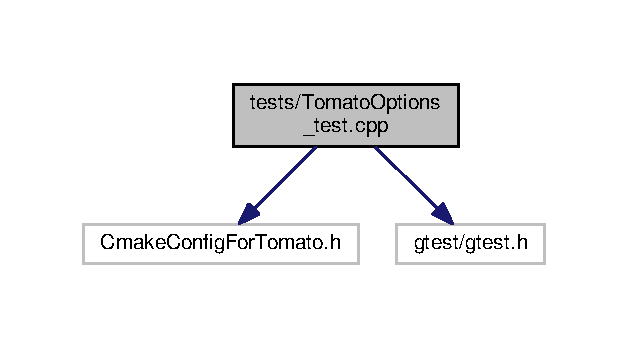
\includegraphics[width=302pt]{_tomato_options__test_8cpp__incl}
\end{center}
\end{figure}


\subsection{Detailed Description}
\begin{DoxyAuthor}{Author}
Konrad Werys 
\end{DoxyAuthor}
\begin{DoxyDate}{Date}
2021/07/05 
\end{DoxyDate}

\input{_tomato_parser__test_8cpp}
\input{_tomato_t1__test_8cpp}
\input{_tomato_t2__test_8cpp}
%--- End generated contents ---

% Index
\backmatter
\newpage
\phantomsection
\clearemptydoublepage
\addcontentsline{toc}{chapter}{Index}
\printindex

\end{document}
